%
% T�TULO DEL CAP�TULO
%
\chapter[Estado do arte]{
	Estado do Arte
	\label{estado_do_arte}
}

Neste cap�tulo analizaremos as diferentes alternativas que existen no mercado como ferramentas de asistencia a traduci�n e as caracteristicas que cada unha incorpora. O final faremos un resumo das caracter�sticas que empregan os programas CAT\footnote{Computer Assisted Translation}.


\section{Internacionalizaci�n � localizaci�n con GNU Gettext}
Gettext � un sistema para a internacionalizaci�n e localizaci�n amplamente usado en entornos UNIX. Conta con var�as implementaci�ns, sendo a primira de Sun Microsystems no ano 1990. A implementaci�n m�is usada � a que GNU liberou no ano 1995.

Pese ser unha soluci�n antiga, � a d�a de hoxe a mellor que se pode atopar no mercado. As s�as principais caracteristicas son:

\paragraph{Soporte de plurales}
Algo que pode parecer trivial como o soporte de plurales deixa de selo cando consideramos que non todos as linguaxes do mundo empregan dous plurales. A lingua eslovaca, por exemplo, conta con tres formas de plural de forma que o plural faise diferente para 1, 3 e 5 elementos.

Gettext representa a forma de plural de cada linguaxe con unha cadea da forma nplurals=n; plural=exp; onde n representa o n�mero de plurais da linguaxe e exp a expresi�n para calcular cando debemos empregar cada forma.

\paragraph{Gardado dos orixes das cadeas}
Gettext almacena para cada cadea en que lugares do c�digo aparece esta. O cal pode ser moi interesante para implentar a previsualizaci�n das traduci�ns.

\paragraph{Comentarios dos programadores}
� unha funci�n moi importante xa que en moitas ocasi�ns nas linguaxes a mesma palabra empregase como verbo ou como nome polo que en ocasi�ns � importante incorporar un contexto para esa traduci�n.

\paragraph{Comentarios dos traductores}
A biblioteca permite que os traductores comenten as cadeas.

\section{Ferramentas CAT do mercado}

Nesta secci�n repasaremos as alternativas existentes no mercado.

\subsection{GTranslator}
GTranslator � a aplicaci�n oficial en GNOME para a traduci�n de arquivos GNU Gettext e so permite abrir este tipo de ficheiros. As caracteristica m�is destacables deste programa son a posibilidade de abrir varios ficheiros en diferentes lapelas, as memorias de traduci�n, perfiles para diferentes traductores, edici�n dos comentarios dos ficheiros .po e un sistema de plugins que permite extender a ferramenta.

\begin{figure}[h]
	\centering
	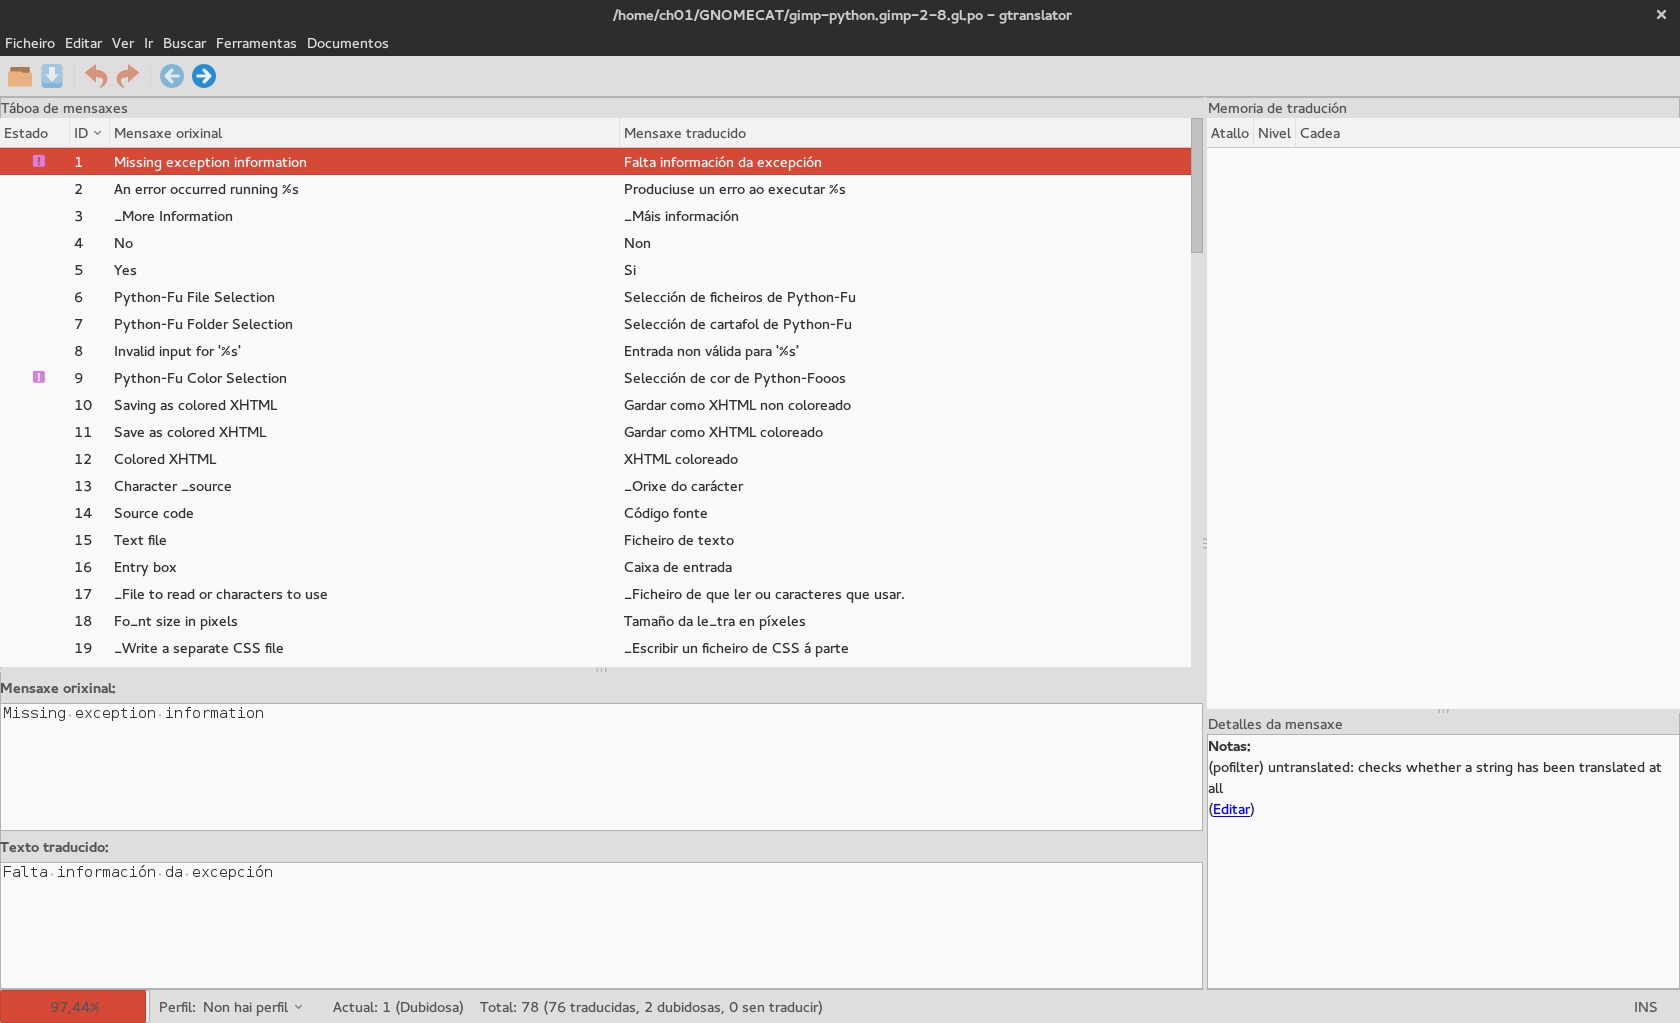
\includegraphics[width=\textwidth]{img/captura_gtranslator.png}
	\caption[Interface de GTranslator]{Interface de GTranslator}
	\label{fig:gtranslator}
\end{figure}

En canto a interface, podemos ver que a parte m�is importante do programa � a a lista de mensaxes. Abaixo temos un panel onde podemos editar cada mensaxe e a dereita a memoria de traduci�n. O programa tam�n incorpora atallos de teclado que permiten moverse polo documento e selecionar cada elemento da memoria de traduci�n.

\subsection{Lokalize}
Lokalize � o programa oficial para a traduci�n en KDE. Ten soporte para ficheiros GNU Gettext e para Qt ts (o formato propio de KDE) entre outros. Entre as caracteristicas a destacar � o soporte para proxectos de traduci�n cunha panel resumo de tod o contido de cada proxecto, ten glosario, memoria de traducion, posibilidade de ver os propios ficheiros fonte desde a interface a trav�s de scripts feitos polo traductor, multiples perfiles, etc.

\begin{figure}[h]
	\centering
	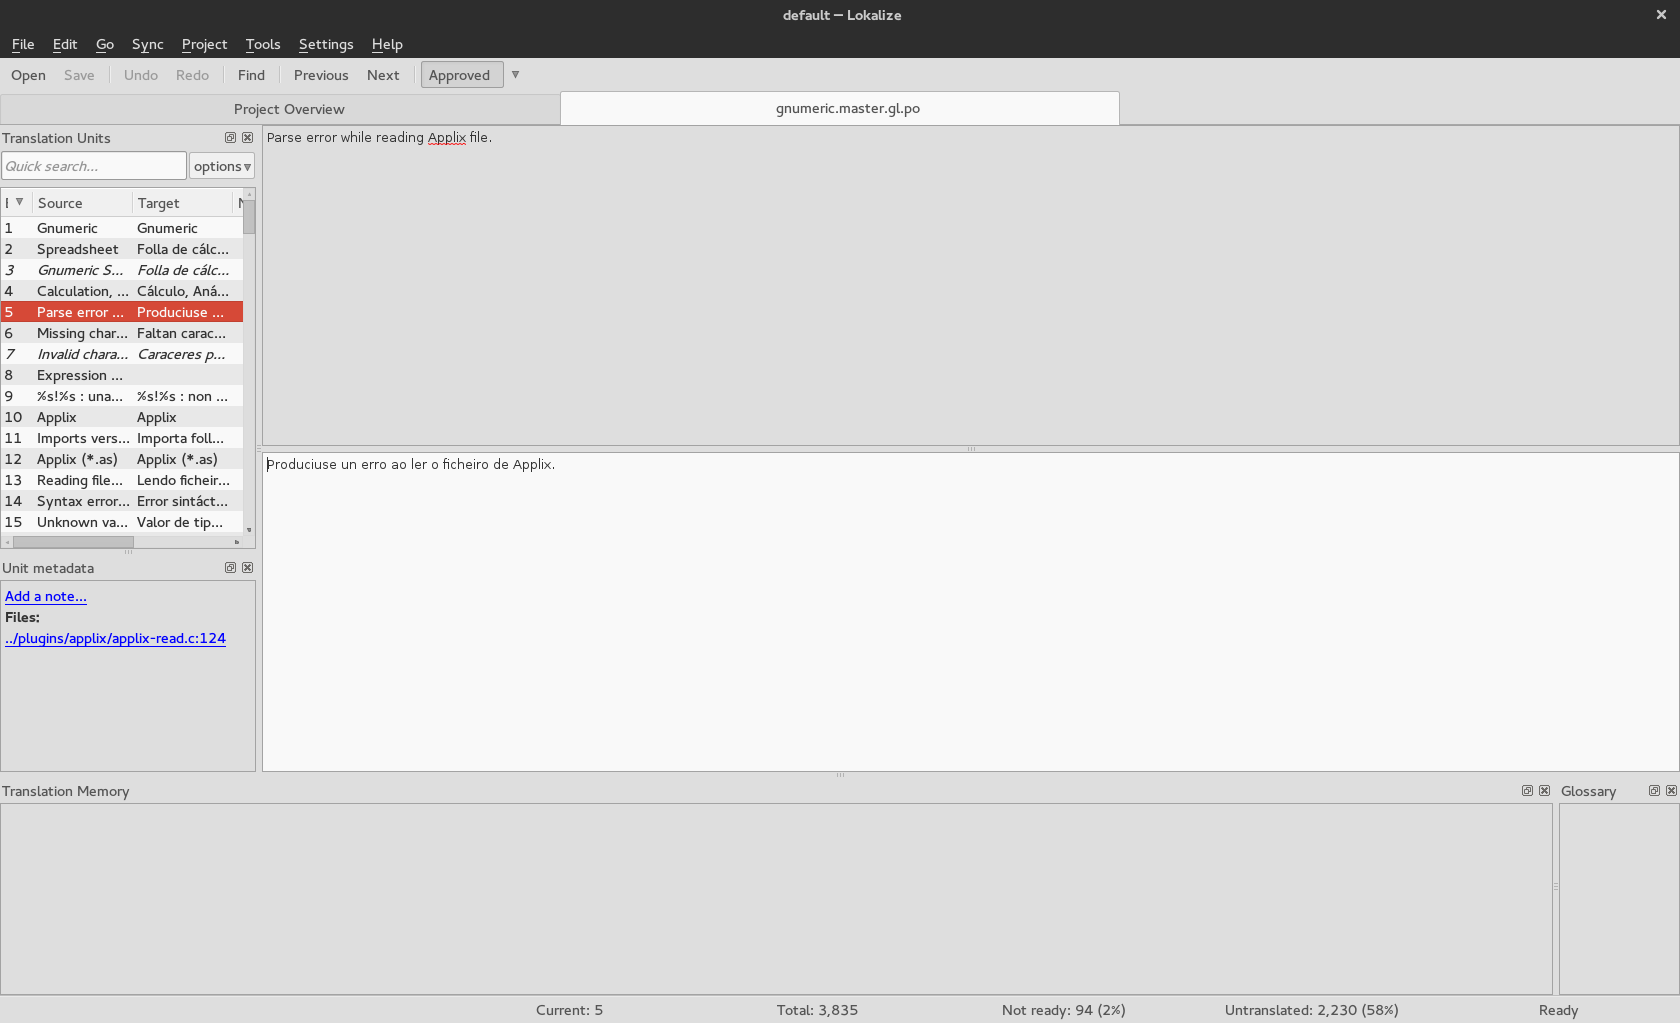
\includegraphics[width=\textwidth]{img/captura_lokalize.png}
	\caption[Interface de Lokalize]{Interface de Lokalize}
	\label{fig:gtranslator}
\end{figure}


\subsection{Virtaal}

\subsection{OmegaT}

\subsection{Google Translation Toolkit}

\subsection{Transifex}


%
% FIN DEL CAP�TULO
%